%
% phdtex
%
% Copyright (c) 2014-2017, Andrew Kanner <andrew.kanner@gmail.com>.
% All rights reserved.
%
% SPDX-License-Identifier: MIT
%

\documentclass[a4paper,12pt]{report}
% добавить leqno в [] для нумерации объектов слева

\IfFileExists{./template/contrib/styles.tex}{\def\template{./template}}{\def\template{.}}

% подключаемые пакеты, стили (в т.ч. ГОСТ Р 7.0.11-2011)
%%% Поля и разметка страницы %%%
\usepackage{lscape}		% Для включения альбомных страниц
\usepackage{geometry}	% Для последующего задания полей

%%% Кодировки и шрифты %%%
\usepackage{cmap}						% Улучшенный поиск русских слов в полученном pdf-файле
\usepackage[T2A]{fontenc}				% Поддержка русских букв (кодировка)
\usepackage[utf8]{inputenc}				% Кодировка utf8 (исходного текста)
\usepackage[english, russian]{babel}	% Языки: русский, английский (локализация и переносы)
\usepackage{pscyr}						% Красивые русские шрифты
\usepackage{extsizes}					% Возможность сделать 14-й шрифт

%%% Альтернативные шрифты %%%
%\usepackage[english, russian]{babel}
%\usepackage{fontspec}					% загрузка шрифтов Open Type, True Type и др.
%\usepackage{euscript}					% Шрифт Евклид
%\usepackage{mathrsfs}					% Красивый матшрифт

%%% Оформление абзацев, колонтитулов, текста %%%
\usepackage{indentfirst}	% Красная строка
\frenchspacing
\usepackage{fancyhdr}		% Колонтитулы
\usepackage{setspace}		% Интерлиньяж

%%% Математические пакеты %%%
\usepackage{amsmath,amsfonts,amssymb,amsthm,mathtools,amscd}	% Математические дополнения от AMS
\usepackage{icomma}												% "Умная" запятая: $0,2$ --- число, $0, 2$ --- перечисление
\usepackage{mathtext}											% русские буквы в формулах
%\usepackage{leqno}												% Нумерация формул слева

%%% Цвета %%%
\usepackage[usenames]{color}
\usepackage{color}
\usepackage{colortbl}
\usepackage[usenames,dvipsnames,svgnames,table,rgb]{xcolor}

%%% Таблицы %%%
\usepackage{array,tabularx,tabulary,booktabs}	% Дополнительная работа с таблицами
\usepackage{longtable}							% Длинные таблицы
\usepackage{multirow,makecell}					% Улучшенное форматирование таблиц (слияние строк и т.п.)

%%% Общее форматирование
\usepackage[singlelinecheck=off,center]{caption}	% Многострочные подписи
\usepackage{soul}									% Поддержка переносоустойчивых подчёркиваний и зачёркиваний
%\usepackage{soulutf8}								% Аналогичные модификаторы начертания

%%% Библиография %%%
\usepackage{cite}				% Красивые ссылки на литературу (библиография)
%\usepackage[superscript]{cite}	% Ссылки в верхних индексах
%\usepackage[nocompress]{cite}
\usepackage{csquotes}			% Еще инструменты для ссылок
%\usepackage[backend=biber,bibencoding=utf8,sorting=ynt,maxcitenames=2,style=authoryear]{biblatex}
%\addbibresource{bib1.bib}
%\usepackage[style=authoryear,maxcitenames=2,backend=biber,sorting=nty]{biblatex}

%%% Гиперссылки %%%
\usepackage[linktocpage=true,plainpages=false,pdfpagelabels=false]{hyperref}

%%% Изображения %%%
\usepackage{graphicx}	% Подключаем пакет работы с графикой
\usepackage{wrapfig}	% Обтекание рисунков текстом

%%% Оглавление %%%
\usepackage{tocloft}

%%% Программирование %%%
\usepackage{etoolbox}	% логические операторы

%%% Рисование
\usepackage{tikz}		% Работа с графикой
\usepackage{pgfplots}
\usepackage{pgfplotstable}

%%% Другие пакеты %%%
\usepackage{lastpage}	% Узнать, сколько всего страниц в документе.
\usepackage{multicol}	% Несколько колонок
\usepackage{totcount}	% Счетчики для глав, приложений и т.д.

%
% phdtex
%
% Copyright (c) 2014-2017, Andrew Kanner <andrew.kanner@gmail.com>.
% All rights reserved.
%
% SPDX-License-Identifier: MIT
%

%% Макет страницы, поля и разметка [перенесено в stylesgost.tex]
%\geometry{a4paper,top=2cm,bottom=2cm,left=3cm,right=1cm}

%% Кодировки и шрифты
% times new roman
\renewcommand{\rmdefault}{ftm}

%% Альтернативные шрифты (см. packages.tex)
% свойства шрифтов по умолчанию
%\defaultfontfeatures{Ligatures={TeX},Renderer=Basic}
% основной шрифт документа
%\setmainfont[Ligatures={TeX,Historic}]{Times New Roman}
% шрифт без засечек
%\setsansfont{Comic Sans MS}
%\setmonofont{Courier New}
% начертание шрифта
%\renewcommand{\familydefault}{\sfdefault}

%% Номера формул
% номера только у тех формул, на которые есть \eqref{} в тексте
%\mathtoolsset{showonlyrefs=true}

%% Выравнивание и переносы
% не допускать переполнений
\sloppy
% запретить разрыв страницы после первой строки абзаца
\clubpenalty=10000
% запретить разрыв страницы после последней строки абзаца
\widowpenalty=10000
% для растягивания или игнорирования "Underfull \hbox"
%\setlength{\emergencystretch}{1pt}
%\sloppy
% глобальные правила переноса (или запрета переноса)
%\hyphenation{сло-во}
% "Overfull", стандартный допустимый: 0.1pt
%\hfuzz=2.5pt
% разреженность, стандартный порог: 200
%\tolerance=400

% кастомные стили для теорем, утверждений и прочего
\newtheoremstyle{plain-indent} % name
{\topsep} % Space above
{\topsep} % Space below
{\itshape} % Body font
%{0pt} % Indent amount
{\parindent} % [New] indent to match GOST
{\bfseries} % Theorem head font
{.} % Punctuation after theorem head
{5pt plus 1pt minus 1pt} % Space after theorem head
{} % Theorem head spec

\newtheoremstyle{definition-indent}
{\topsep}
{\topsep}
{\normalfont} % diff
%{0pt}
{\parindent}
{\bfseries}
{.}
{5pt plus 1pt minus 1pt}
{}

\newtheoremstyle{remark-indent}
{0.5\topsep} % diff
{0.5\topsep} % diff
{\normalfont} % diff
%{0pt}
{\parindent}
{\itshape} % diff
{.}
{5pt plus 1pt minus 1pt}
{}

%% Математические конструкции (теоремы, утверждения и т.д.)
% стиль по умолчанию
\theoremstyle{plain-indent}
\newtheorem{theorem}{Теорема}
\newtheorem{proposition}{Утверждение}
\newtheorem{lemma}{Лемма}
% стиль определений
\theoremstyle{definition-indent}
\newtheorem{corollary}{Следствие}
\newtheorem{problem}{Задача}[section]
\newtheorem{condition}{Условие}
\newtheorem{definition}{Определение}
\newtheorem{axiom}{Аксиома}
% стиль примечаний
\theoremstyle{remark-indent}
\newtheorem*{nonum}{Решение}

%% Цветовые эффекты (выделение текста)
\newcommand\hly[1]{\colorbox{yellow!80}{\begin{varwidth}{\dimexpr\linewidth-2\fboxsep}#1\end{varwidth}}}
\newcommand\hlg[1]{\colorbox{green!80}{\begin{varwidth}{\dimexpr\linewidth-2\fboxsep}#1\end{varwidth}}}
% цветные текст-боксы для таблиц и графиков
\newcommand\hlyy[1]{\fcolorbox{black!50}{yellow!25}{\begin{varwidth}{\dimexpr\linewidth-2\fboxsep}#1\end{varwidth}}}
\newcommand\hlgg[1]{\fcolorbox{black!50}{green!25}{\begin{varwidth}{\dimexpr\linewidth-2\fboxsep}#1\end{varwidth}}}
\newcommand\hlbrr[1]{\fcolorbox{black!50}{brown!25}{\begin{varwidth}{\dimexpr\linewidth-2\fboxsep}#1\end{varwidth}}}
\newcommand\hlbll[1]{\fcolorbox{black!50}{black!25}{\begin{varwidth}{\dimexpr\linewidth-2\fboxsep}#1\end{varwidth}}}
\newcommand\hlrr[1]{\fcolorbox{black!50}{red!25}{\begin{varwidth}{\dimexpr\linewidth-2\fboxsep}#1\end{varwidth}}}
\newcommand\hlbluu[1]{\fcolorbox{black!50}{blue!25}{\begin{varwidth}{\dimexpr\linewidth-2\fboxsep}#1\end{varwidth}}}
\newcommand\hlempty[1]{\fcolorbox{black!50}{white}{\begin{varwidth}{\dimexpr\linewidth-2\fboxsep}#1\end{varwidth}}}
\newcommand\hlbr[1]{\colorbox{brown!80}{\begin{varwidth}{\dimexpr\linewidth-2\fboxsep}#1\end{varwidth}}}
\newcommand\hlbl[1]{\colorbox{black!80}{\begin{varwidth}{\dimexpr\linewidth-2\fboxsep}#1\end{varwidth}}}
\newcommand\hlr[1]{\colorbox{red!80}{\begin{varwidth}{\dimexpr\linewidth-2\fboxsep}#1\end{varwidth}}}
\newcommand\hlblu[1]{\colorbox{blue!80}{\begin{varwidth}{\dimexpr\linewidth-2\fboxsep}#1\end{varwidth}}}
% deprecated вариант2
% \newcommand\hl{\bgroup\markoverwith{\textcolor{yellow}{\rule[-.5ex]{2pt}{2.5ex}}}\ULon}
% deprecated вариант3
%\newcommand*{\hl}[1]{\colorbox{yellow}{#1}}

%% Изображения
% путь к каталогу с изображениями
\graphicspath{{images/}}
% отступ рамки \fbox{} от рисунка
\setlength\fboxsep{3pt}
% толщина линий рамки \fbox{}
\setlength\fboxrule{1pt}

%% Библиография
\makeatletter
% библиография в соответствии с ГОСТ 7.1-2003
\bibliographystyle{\template/contrib/utf8gost71my}
% заменить квадратные скобки на точку
\renewcommand{\@biblabel}[1]{#1.}
\makeatother

%% Гиперссылки: цвета и другие настройки
\definecolor{linkcolor}{rgb}{0.9,0,0}
\definecolor{citecolor}{rgb}{0,0.6,0}
\definecolor{urlcolor}{rgb}{0,0,1}
\hypersetup{
  % русские буквы в разделах
  unicode=true,
  % true: цветные ссылки; false: ссылки в рамках
  colorlinks=true,
  % внутренние ссылки
  linkcolor={linkcolor},
  % ссылки на библиографию
  citecolor={citecolor},
  % на файлы
  filecolor=magenta,
  % на URL
  urlcolor={urlcolor}
}

%% Оглавление
\renewcommand{\cftchapdotsep}{\cftdotsep}


%% Листинги
% стиль javascript
\lstdefinelanguage{JavaScript}{
  keywords={break, case, catch, continue, debugger, default, delete,
    do, else, false, finally, for, function, if, in, instanceof, new,
    null, return, switch, this, throw, true, try, typeof, var, void,
    while, with},
  comment=[l]{//},
  morecomment=[s]{/*}{*/},
  morestring=[b]',
  morestring=[b]",
  ndkeywords={class, export, boolean, throw, implements, import,
    this},
  keywordstyle=\color{blue}\bfseries,
  ndkeywordstyle=\color{yellow}\bfseries,
  identifierstyle=\color{black},
  commentstyle=\color{green}\ttfamily,
  stringstyle=\color{red}\ttfamily
  sensitive=true,
}
% стиль xml
\lstdefinelanguage{xml}{
  morekeywords={name,description,memory,unit,os,arch,machine,devices,emulator,hostdev,
    mode, type, managed, source, vendor, id, product, address, domain,
    bus, slot, function},
  numbers=none,
  frame=none,
  belowskip=2pt,
  caption=,
}
% стиль bash
\lstdefinelanguage{bashhh}{
  morekeywords={modprobe,echo},
  deletekeywords={bind},
  morecomment=[l]{\#},
  numbers=none,
  frame=none,
  belowskip=2pt,
  caption=,
}
% цветовая схема для выделения блоков кода
\definecolor{codegreen}{rgb}{0,0.6,0}
\definecolor{codegray}{rgb}{0.5,0.5,0.5}
\definecolor{codemauve}{rgb}{0.58,0,0.82}
\lstset{
  % язык программирования [должен выставляться в самом листинге!]
  % language=C,
  % language=JavaScript,
  % моноширинный шрифт
  columns=fixed,
  % цвет фона (использует пакеты color/xcolor)
  backgroundcolor=\color{white},
  % размер и начертание
  basicstyle=\small\sffamily,
  % перенос строки только при наличии пробела
  breakatwhitespace=false,
  % автоматический перенос строк
  breaklines=true,
  % позиция заголовка (вверху: t, внизу: b)
  captionpos=b,
  % стиль для комментариев
  commentstyle=\color{codegreen},
  % стиль для ключевых слов
  keywordstyle=\color{blue},
  % дополнительные ключевые слова
  morekeywords={*,...},
  % можно удалить какие-нибудь ключевые слова
  deletekeywords={...},
  % для использования latex в коде
  escapeinside={\%*}{*)},
  % разрешить использовать не-ASCII символы
  extendedchars=true,
  % extendedchars=\true,
  % inputencoding=utf8x,
  % keepspaces = true,
  % добавить рамку вокруг кода
  frame=single,
  % если не установлено, то цвет рамки может меняться
  rulecolor=\color{black},
  % позиция номеров строк
  numbers=left,
  % расстояние от номера строки до кода
  numbersep=5pt,
  % размер шага между номерами строк
  stepnumber=1,
  % стиль для номеров строк
  numberstyle=\tiny\color{codegray},
  % не показывать пробелы в виде отступов
  showspaces=false,
  % не показывать пробелы в строках
  showstringspaces=false,
  % не показывать знаки табуляции
  showtabs=false,
  % стиль для строковых литералов
  stringstyle=\color{codemauve},
  % размер табуляции
  tabsize=2,
  % показывать имя подключаемого файла
  title=\lstname
}

%% Разное
% использовать \slash для переноса слов, разделенных "\"?

%%% Колонтитулы (см. packages.tex) %%%
\pagestyle{fancy}
\renewcommand{\headrulewidth}{0pt}	% Толщина линейки, отчеркивающей верхний колонтитул
%\lfoot{Нижний левый}
%\rfoot{Нижний правый}
%\rhead{Верхний правый}
%\chead{Верхний в центре}
%\lhead{Верхний левый}
%\cfoot{Нижний в центре}			% По умолчанию здесь номер страницы
\lfoot{}
\rfoot{}
\rhead{}
\chead{\normalsize\thepage}
\lhead{}
\cfoot{}

%%% при использовании chapters - первая страница создается в plain pagestyle %%%
\fancypagestyle{plain}{\pagestyle{fancy}}

%%% Интерлиньяж %%%
\onehalfspacing	% Интерлиньяж 1.5
%\doublespacing	% Интерлиньяж 2
%\singlespacing	% Интерлиньяж 1

%%% Макет страницы %%%
\geometry{a4paper,top=20mm,bottom=20mm,left=25mm,right=10mm}

\usepackage{sectsty}
\allsectionsfont{\centering}	% центрирование заголовков (должны быть без точки на конце и переносов)

%%% список сокращений %%%
\usepackage{nomencl}

% Позволяет одновременно печатать условное обозначение в тексте документа и добавлять его в перечень
\newcommand*{\nom}[2]{#1\nomenclature{#1}{#2}}

%%% Формат формул и ссылок на формулы %%%
% ПРИМЕР:
%\begin{equation}\label{name}
%	2+2=4
%\end{equation}
%
%Формула \eqref{name}

% Перечень сокращений будет распечатываться по алфавиту вне зависимости от появления в тексте
% ПРИМЕР:
%\nom{Б}{Вторая буква алфавита}.
%А\nomenclature{А}{Первая буква алфавита}

% Список литературы формируется в порядке возрастания - bib1, bib2, bib3,...
% по ГОСТ НЕОБХОДИМО, чтобы источники на отличном от русского языке перечислялись ПОСЛЕ источников на русском

% Приложения ДОЛЖНЫ быть перечислены в порядке их перечисления в тексте

% добавим файл с информацией по работе, автору и т.д.
% !TEX root = dissertation.tex synopsis.tex

%
% phdtex
%
% Copyright (c) 2014-2020, Andrew Kanner <andrew.kanner@gmail.com>.
% All rights reserved.
%
% SPDX-License-Identifier: CC-BY-4.0
%

% заголовок
\author{ФАМИЛИЯ ИМЯ ОТЧЕСТВО автора}
\title{НАЗВАНИЕ ДИССЕРТАЦИОННОЙ РАБОТЫ}

% неизменяемые общие данные
\date{\today}
\makeatletter
\def\dissauthor{\@author}
\def\disstitle{\@title}
\def\dissdate{\@date}
\makeatother
\def\dissyear{\the\year}

% специальность, ученая степень, руководитель, консультант, оппоненты
\def\specnum{ХХ.ХХ.ХХ}
\def\specname{<<Название специальности>>}
\def\edudegree{кандидата каких-то там наук}
\def\mentordegree{уч. степень, уч. звание}
%\def\mentortitle{уч. звание}
\def\mentorcompany{Название\\компании,\\г. Город\\~}
\def\mentorname{Фамилия И. О.}
\def\consultantdegree{уч. степень}
\def\consultantcompany{Название компании,\\ г. Город}
\def\consultantname{Фамилия И. О.}
\def\opponentonedegree{уч. степень}
\def\opponentonecompany{\\Название компании,\\ г. Город}
\def\opponentonename{Фамилия И. О.}
\def\opponenttwodegree{уч. степень}
\def\opponenttwocompany{\\Название компании,\\ г. Город}
\def\opponenttwoname{Фамилия И. О.}
\def\opponentthreedegree{уч. степень}
\def\opponentthreecompany{\\Название компании,\\ г. Город}
\def\opponentthreename{Фамилия И. О.}
\def\leadingorg{Название ведущей организации}

% прочие данные
\def\disscity{Город }
\def\dissorg{НАЗВАНИЕ УЧРЕЖДЕНИЯ, В КОТОРОМ ВЫПОЛНЯЛАСЬ\par
ДАННАЯ ДИССЕРТАЦИОННАЯ РАБОТА\par}
\def\dissorgsyn{<<Название учреждения, в котором выполнялась данная
  диссертационная работа>>}
\def\dissudk{УДК xxx.xxx}

% данные для оборота титульного листа автореферата
\def\councildate{<<\dots>> \dots \the\year~г.}
\def\counciltime{\dots:00}
\def\councilnum{Д xxx.xxx.xx}
\def\councilplace{<<Организация, к которой относится диссертационный
  совет>>}
\def\counciladdress{Индекс, г.~Город, шоссе / улица / \dots,~д.xx}
\def\libraryname{<<Организация, куда передается рукопись
  диссертационной работы>> и на сайте:}
\def\libraryaddress{Индекс, г.~Город, шоссе / улица / \dots,~д.xx}
\def\councilwebsite{http://website.ru}
\def\synopsissentdate{<<\dots>> \dots \the\year~года}
\def\councilsecretarydegree{уч. степень, уч. звание}
\def\councilsecretaryname{И.О.~Фамилия}

% выставим атрибуты pdf-документа
\hypersetup{
  % заголовок
  pdftitle={\disstitle},
  % автор
  pdfauthor={\dissauthor},
  % тема
  pdfsubject={\disstitle},
  % создатель
  pdfcreator={\dissauthor},
  % производитель
  pdfproducer={\dissauthor},
  % ключевые слова
  pdfkeywords={keyword1} {keyword2}
}


% \includeonly{01-title, \template/contrib/contents, parts/intro,
% parts/references}

% включить для проверки вхождения всех источников в текст (см. в конце)
%\usepackage{refcheck}

% нужно будет сделать список сокращений и условных обозначений
\makenomenclature

\begin{document}

% переопределение именований
%
% phdtex
%
% Copyright (c) 2014-2017, Andrew Kanner <andrew.kanner@gmail.com>.
% All rights reserved.
%
% SPDX-License-Identifier: MIT
%

% переопределение именований
\renewcommand{\abstractname}{Аннотация}
\renewcommand{\alsoname}{см. также}
\renewcommand{\appendixname}{Приложение}
\renewcommand{\bibname}{Список использованных источников}
\renewcommand{\ccname}{исх.}
\renewcommand{\chaptername}{Глава}
\renewcommand{\contentsname}{Содержание}
\renewcommand{\enclname}{вкл.}
\renewcommand{\figurename}{Рисунок}
\renewcommand{\headtoname}{вх.}
\renewcommand{\indexname}{Предметный указатель}
\renewcommand{\listfigurename}{Список рисунков}
\renewcommand{\listtablename}{Список таблиц}
\renewcommand{\pagename}{Стр.}
\renewcommand{\partname}{Часть}
\renewcommand{\refname}{Список литературы}
\renewcommand{\seename}{см.}
\renewcommand{\tablename}{Таблица}
\renewcommand{\lstlistingname}{Листинг}

% заголовок перечня nomenclature
\renewcommand{\nomname}{Перечень сокращений и условных обозначений}

% переопределение математических символов на русский манер
\renewcommand{\epsilon}{\ensuremath{\varepsilon}}
\renewcommand{\phi}{\ensuremath{\varphi}}
\renewcommand{\kappa}{\ensuremath{\varkappa}}
\renewcommand{\le}{\ensuremath{\leqslant}}
\renewcommand{\leq}{\ensuremath{\leqslant}}
\renewcommand{\ge}{\ensuremath{\geqslant}}
\renewcommand{\geq}{\ensuremath{\geqslant}}
\renewcommand{\emptyset}{\varnothing}

% перенос знаков в формулах (по Львовскому)
\newcommand*{\hm}[1]{#1\nobreak\discretionary{}
{\hbox{$\mathsurround=0pt #1$}}{}}

% сокращения
\newcommand*{\linux}{GNU/Linux}
\newcommand*{\linuxkernel}{Linux}

% дополнительные команды
%\DeclareMathOperator{\sgn}{\mathop{sgn}}
\newcommand*{\nbline}{\\*\indent}
\newcommand{\tab}[1]{\hspace{.1\textwidth}\rlap{#1}}
\newcommand*{\ti}[1]{\text{\textit{#1}}}

% счетчик для пунктов в первом столбце таблиц
\newcounter{rowcount}
\setcounter{rowcount}{0}
\newcommand\rownumber{\stepcounter{rowcount}\arabic{rowcount}.}


% титульный лист
% !TEX root = dissertation.tex

%
% phdtex
%
% Copyright (c) 2014-2017, Andrew Kanner <andrew.kanner@gmail.com>.
% All rights reserved.
%
% SPDX-License-Identifier: MIT
%

\thispagestyle{empty}

\begin{center}
\dissorg
\par
\end{center}

\vspace{10mm}
\begin{flushright}
На правах рукописи

{\sl \dissudk}
\end{flushright}

\vspace{20mm}
\begin{center}
{\large \dissauthor}
\end{center}

\vspace{5mm}
\begin{center}
{\bf \large \disstitle
\par}

\vspace{10mm}
{%\small
Специальность \specnum~---

\specname
}

\vspace{10mm}
Диссертация на соискание ученой степени

\edudegree
\end{center}

\vspace{5mm}
\begin{flushright}
Научный руководитель:

\mentordegree

\mentorname
\end{flushright}

%\vspace{1mm}
\begin{flushright}
Научный консультант:

\consultantdegree

\consultantname

\end{flushright}

\vfill
\begin{center}
{\disscity -- \dissyear}
\end{center}

%\newpage
\resetHeadWidth

% оглавление
\tableofcontents
\clearpage


% текст введения находится в introduction.tex
% !TEX root = ../dissertation.tex

% вынесено из 02-introduction.tex с целью использования разных
% заголовков в автореферате и тексте диссертации

% заголовок
\begin{singlespace}
  \chapter*{\MakeUppercase{Введение}}
\end{singlespace}
% добавляем введение в оглавление
\addcontentsline{toc}{chapter}{Введение}

% введение
% !TEX root = dissertation.tex

\chapter*{Введение}							% Заголовок
\addcontentsline{toc}{chapter}{Введение}	% Добавляем его в оглавление
Обзор, введение в тему, обозначение места данной работы в мировых исследованиях и т.п.

\textbf{Целью} данной работы является \ldots

Для~достижения поставленной цели необходимо было решить следующие задачи:
\begin{enumerate}
  \item Исследовать, разработать, вычислить и т.д. и т.п.
  \item Исследовать, разработать, вычислить и т.д. и т.п.
  \item Исследовать, разработать, вычислить и т.д. и т.п.
  \item Исследовать, разработать, вычислить и т.д. и т.п.
\end{enumerate}

\textbf{Основные положения, выносимые на~защиту:}
\begin{enumerate}
  \item Первое положение
  \item Второе положение
  \item Третье положение
  \item Четвертое положение
\end{enumerate}

\textbf{Научная новизна:}
\begin{enumerate}
  \item Впервые \ldots
  \item Впервые \ldots
  \item Было выполнено оригинальное исследование \ldots
\end{enumerate}

\textbf{Научная и практическая значимость} \ldots

\textbf{Степень достоверности} полученных результатов обеспечивается \ldots Результаты находятся в соответствии с результатами, полученными другими авторами.

\textbf{Апробация работы.}
Основные результаты работы докладывались~на:
перечисление основных конференций, симпозиумов и т.п.

\textbf{Личный вклад.} Автор принимал активное участие \ldots

\textbf{Публикации.} Основные результаты по теме диссертации изложены в ХХ печатных изданиях~\cite{bib1,bib2,bib3,bib4,bib5},
Х из которых изданы в журналах, рекомендованных ВАК~\cite{bib1,bib2,bib3}, 
ХХ --- в тезисах докладов~\cite{bib4,bib5}.

\textbf{Объем и структура работы.} Диссертация состоит из~введения, \total{chapnum} глав, заключения и~\total{appendnum} приложени\hly{я}. Полный объем диссертации составляет \pageref{LastPage}~страниц\hly{ы} с~\hly{ХХ}~рисунками и~\hly{ХХ}~таблицами. Количество наименований в списке литературы --- \total{bibnum}.

%\clearpage

% главы 1-4, заключение
% !TEX root = dissertation.tex

%
% phdtex
%
% Copyright (c) 2014-2017, Andrew Kanner <andrew.kanner@gmail.com>.
% All rights reserved.
%
% SPDX-License-Identifier: CC-BY-4.0
%

\begin{singlespace}
  \realchapter{Название главы 1} \label{chapt1}
\end{singlespace}

% комментарии разработчика шаблона
Для более удобного использования cvs типа git лучше использовать
редактор с переносом строк длиной более 80 символов. Так будет проще
вносить и затем просматривать изменения по длинным абзацам.

Перенос строк в latex не является признаком начала нового абзаца,
новый абзац начинается если перед текстом вставлена пустая строка (как
перед этим предложением). \\

\section{Название раздела 1.1} \label{sect1_1}

Текст раздела \dots{} \\

Нумерованный список:
\begin{enumerate}
\item пункт 1;
\item пункт 2;
\item пункт 3. \\
\end{enumerate}

Ненумерованный список:
\begin{itemize}
\item пункт 1;
\item пункт 2;
\item пункт 3. \\
\end{itemize}

Список c произвольными разделителями:
\begin{description}
\item{\textbf{[п1]}} пункт 1;
\item{\textbf{[п2]}} пункт 2;
\item{\textbf{[п3]}} пункт 3. \\
\end{description}

Совмещенные списки:
\begin{enumerate}
\item пункт 1:
      \begin{itemize}
      \item подпункт 1.
      \end{itemize}
\item пункт 2;
\item пункт 3. \\
\end{enumerate}

Список myenumerate (см. contrib/stylesgost.tex):
\begin{myenumerate}
\item пункт 1;

  Дополнительный длинный-длинный-длинный текст без изменения
  форматирования по отношению к основному тексту вне списка.

\item пункт 2;
\item пункт 3. \\
\end{myenumerate}

Пример рисунка (см. Рисунок \ref{test1}). \\

\begin{figure}[bhtp]
  \centering 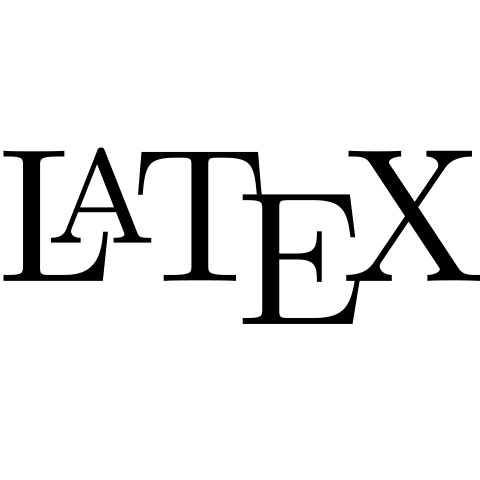
\includegraphics[scale=0.1]{latex-cc0}
  \caption{Подпись рисунка} \label{test1}
\end{figure}

Символ\_подчеркивания, символ процента -- \%. \\

Числа вводятся в math mode: $1$, $2$, $3$ \dots{} \\

Запрет переноса специфических терминов, неразрывный пробел:
\mbox{идентификация/аутентификация} или \mbox{ФСТЭК},
эту~фразу~переносить~нельзя
(только~целиком~или~по~правилам~переносов~слов). \\

Сокращения и условные обозначения: операционная система
(\nom{ОС}{Операционная система}). \\

<<Правильные>> кавычки. Правильное тире --, теперь длинное ---. \\

Выделения текста: \textbf{bold}, \textit{italic},
\underline{underline}, \hly{цветом}, \dots{} \\

Ссылки: литературные источники \cite{article_other}, несколько вместе
\cite{article_pub, article_vak, article_scopus, book1, thesis1,
  conference1, hyperlink1}; сноски\footnote{Текст сноски.}; ссылки на
любые помеченные сущности с помощью label, например на главу
\ref{chapt1}, ссылки на страницу с помеченной сущностью
\pageref{chapt1}. \\

\subsection{Подраздел} \label{subsect1_1_1}

\subsubsection{<<Подподраздел>>} \label{subsect1_1_1_1}

% этот label используется для простановки номеров страниц в Положениях
% из введения
Конец раздела.\label{sect1_1-eof}

%\newpage
%===============================================================================

\section{Название раздела 1.2} \label{sect1_2}

%\newpage
%===============================================================================

\section{Выводы} \label{sect1_3}

\begin{enumerate}
\item Вывод 1.
\item Вывод 2.
\item Вывод 3.
\end{enumerate}

%\clearpage

\chapter{Длинное название главы, в которой мы смотрим на примеры того, как будут верстаться изображения и списки} \label{chapt2}

\section{Одиночное изображение} \label{sect2_1}

\begin{figure} [h] 
  \center
%  \includegraphics [scale=0.27] {LaTeX}
	
\includegraphics [scale=0.27] {latex}
  \caption{TeX.} 
  \label{img:latex}  
\end{figure}

%\newpage
%============================================================================================================================
\section{Длинное название параграфа, в котором мы узнаём как сделать две картинки с общим номером и названием} \label{sect2_2}

А это две картинки под общим номером и названием:
\begin{figure}[h]
  \begin{minipage}[h]{0.49\linewidth}
    \center{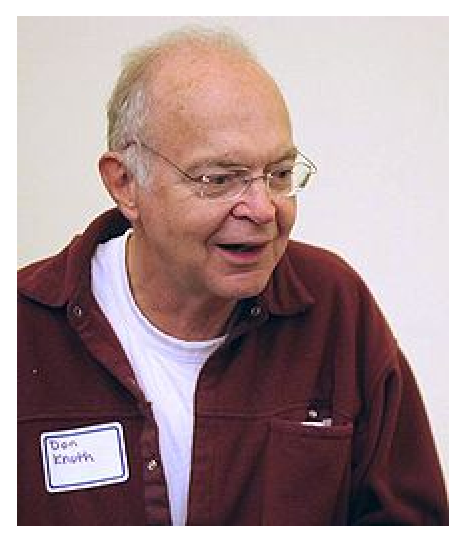
\includegraphics[width=0.5\linewidth]{knuth1} \\ а)}
  \end{minipage}
  \hfill
  \begin{minipage}[h]{0.49\linewidth}
    \center{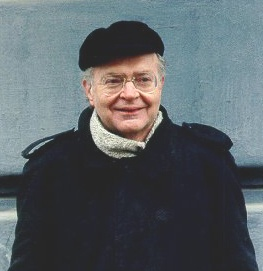
\includegraphics[width=0.5\linewidth]{knuth2} \\ б)}
  \end{minipage}
  \caption{Очень длинная подпись к изображению, на котором представлены две фотографии Дональда Кнута}
  \label{img:knuth}  
\end{figure}

%\newpage
%============================================================================================================================
\section{Пример вёрстки списоков} \label{sect2_3}

\noindent Нумерованный список:
\begin{enumerate}
  \item Первый пункт.
  \item Второй пункт.
  \item Третий пункт.
\end{enumerate}

\noindent Маркированный список:
\begin{itemize}
  \item Первый пункт.
  \item Второй пункт.
  \item Третий пункт.
\end{itemize}

\noindent Вложенные списки:
\begin{itemize}
  \item Имеется маркированный список.
  \begin{enumerate}
    \item В нём лежит нумерованный список,
    \item в котором
    \begin{itemize}
      \item лежит ещё один маркированный список.
    \end{itemize}    
  \end{enumerate}
\end{itemize}


\clearpage

% !TEX root = dissertation.tex

\chapter{Вёрстка таблиц} \label{chapt3}

\section{Таблица обыкновенная} \label{sect3_1}

Так размещается таблица:

\begin{table} [htbp]
  \centering
  \parbox{15cm}{\caption{Название таблицы}\label{Ts0Sib}}
%  \begin{center}
  \begin{tabular}{| p{3cm} || p{3cm} | p{3cm} | p{4cm}l |}
  \hline
  \hline
  Месяц   & \centering $T_{min}$, К & \centering $T_{max}$, К &\centering  $(T_{max} - T_{min})$, К & \\
  \hline
  Декабрь &\centering  253.575   &\centering  257.778    &\centering      4.203  &   \\
  Январь  &\centering  262.431   &\centering  263.214    &\centering      0.783  &   \\
  Февраль &\centering  261.184   &\centering  260.381    &\centering     $-$0.803  &   \\
  \hline
  \hline
  \end{tabular}
%  \end{center}
\end{table}

%\newpage
%============================================================================================================================

\section{Параграф - два} \label{sect3_2}

Некоторый текст.

%\newpage
%============================================================================================================================

\section{Параграф с подпараграфами} \label{sect3_3}

\subsection{Подпараграф - один} \label{subsect3_3_1}

Некоторый текст.

\subsection{Подпараграф - два} \label{subsect3_3_2}

Некоторый текст.

%\clearpage
% !TEX root = dissertation.tex

\begin{singlespace}
  \realchapter{Название главы 4} \label{chapt4}
\end{singlespace}

\section{Название раздела 4.1} \label{sect4_1}

Какой-нибудь график и другие результаты экспериментальных исследований
(см. рисунок~\ref{test-tikz}).

\begin{figure}[h!]
  \centering
  \begin{tikzpicture}
    \begin{axis}[width=0.6\textwidth, height=0.7\textwidth, xmin=0,
      xmax=6, ymin=0, ymax=100, ytick={0,100}, yticklabels={0,100\%},
      xtick={0,1,2,3,4,5,6}, xticklabels={, $2012$, $2013$, $2014$,
        $2015$, $2016$, гг.},]

      \addplot[name path=axs1, white] coordinates {(1,99)
        (5,99)};

      \addplot[name path=plt1,red!80,smooth,ultra thick] coordinates {
        (1,50) (2,60) (3,75) (4,85) (5,99) };

      \addplot[black] fill between[of=plt1 and axs1, split, every
      segment no 0/.style={pattern color=red!20, pattern=north east
        lines}, every segment no 1/.style={pattern color=red!20,
        pattern=north east lines}, ];

      \end{axis}
    \end{tikzpicture}

    \caption{Подпись к графику}
      \label{test-tikz}

\end{figure}

%\newpage
%===============================================================================

\section{Название раздела 4.2} \label{sect4_2}

Про апробацию и внедрение, покрытие статьями текста диссертации,
личный вклад автора \dots{}

Возможные направления дальнейших исследований по данной теме.

%\newpage
%===============================================================================

\section{Выводы} \label{sect4_3}

\begin{enumerate}
\item Вывод 1.
\item Вывод 2.
\item Вывод 3.
\end{enumerate}

%\clearpage

% !TEX root = dissertation.tex

%
% phdtex
%
% Copyright (c) 2014-2017, Andrew Kanner <andrew.kanner@gmail.com>.
% All rights reserved.
%
% SPDX-License-Identifier: CC-BY-4.0
%

\begin{singlespace}
  \chapter*{\MakeUppercase{Заключение}}
\end{singlespace}

% добавляем заключение в оглавление
\addcontentsline{toc}{chapter}{Заключение}

Основные результаты работы, заключаются в следующем:

\begin{enumerate}
\item Проведен анализ \dots{} исследовано \dots{} предложено \dots{}
\item Сформированы \dots{}.
\item На базе полученных научных результатов разработано \dots{}
\item В ходе экспериментальных исследований подтвержден ожидаемый
  эффект от применения \dots{}, а также соответствие \dots{}.
\end{enumerate}

%\clearpage


% списки таблиц и изображений
% !TEX root = ../dissertation.tex

\clearpage
\phantomsection \addcontentsline{toc}{chapter}{\listfigurename}
% список изображений
\listoffigures
\newpage

\clearpage
\phantomsection \addcontentsline{toc}{chapter}{\listtablename}
% cписок таблиц
\listoftables
\newpage

\clearpage
\phantomsection \addcontentsline{toc}{chapter}{\nomname}
% список сокращений и условных обозначений
\printnomenclature
\newpage
% список литературы
% !TEX root = ../dissertation.tex

%
% phdtex
%
% Copyright (c) 2014-2017, Andrew Kanner <andrew.kanner@gmail.com>.
% All rights reserved.
%
% SPDX-License-Identifier: MIT
%

\clearpage
\phantomsection
% добавляем список литературы в оглавление
\addcontentsline{toc}{chapter}{\bibname}
% подключаем bibtex-файлы
\bibliography{parts/biblio,parts/biblio-pub,parts/biblio-vak}

% приложения
% !TEX root = ../dissertation.tex

\appendix
\appndchapter{Название первого приложения} \label{AppendixA}

Текст приложения

%\clearpage

% раскомментировать для пометки не вошедших источников из bibtex-баз
%\nocite{*}

\end{document}
